% file: bivalent-init-b-solo.tex

\documentclass{standalone}

\usepackage{tikz}
\usetikzlibrary{positioning, arrows.meta, decorations.pathreplacing}

\begin{document}
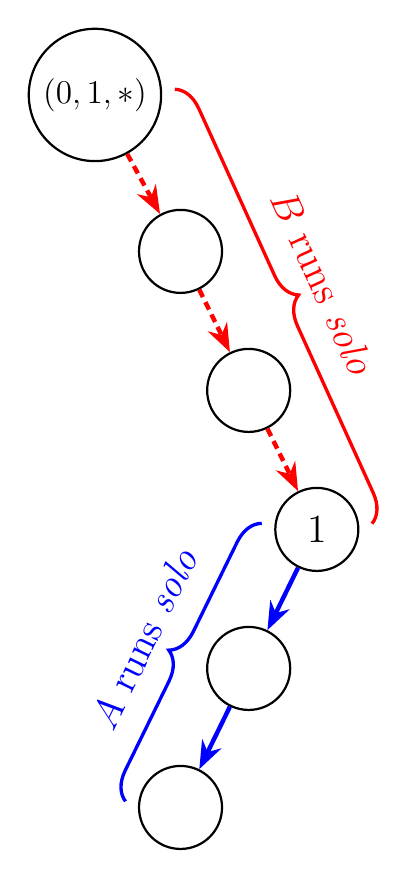
\begin{tikzpicture}[state/.style = {draw, thick, circle, minimum size = 30pt},
  move/.style = {draw, ultra thick, >=Stealth, ->},
  amove/.style = {move, blue},
  bmove/.style = {move, red, densely dashed}]
  \node (r) [state, font = \large] {$(0,1,\ast)$};

  \foreach \p/\c/\v in {r/b1/, b1/b2/, b2/b3/1} {
    \node (\c) [state, below right = 1.00cm and 0.1cm of \p, font = \Large] {$\v$};
    \draw [bmove] (\p) to (\c);
  }

  \foreach \p/\c in {b3/a1, a1/a2} {
    \node (\c) [state, below left = 1.00cm and 0.1cm of \p] {};
    \draw [amove] (\p) to (\c);
  }

  \draw [decorate, red, very thick, decoration = {brace, amplitude = 10pt, raise = 5pt}] 
    (r.east) -- (b3.east) node [midway, sloped, above = 16pt, font = \Large] {$B$ runs \emph{solo}};

  \draw [decorate, blue, very thick, decoration = {brace, mirror, amplitude = 10pt, raise = 5pt}] 
    (b3.west) -- (a2.west) node [midway, sloped, above = 16pt, font = \Large] {$A$ runs \emph{solo}};
\end{tikzpicture}
\end{document}
